\chapter{Design of a User Study}
\label{chapter5}
\thispagestyle{empty}

\begin{quotation}
{\footnotesize
\noindent{\emph{``\greek{`p'antwn qrhm'atwn m'etron', >'anjrwpon e>~inai, 't~wn m`en >'ontwn <wc >'esti, t~wn d`e m`h >'ontwn <wc o>uk >'estinv.'}''}\\
(man is \textquotedblleft the measure of all things, of the existence of the things that are and the non-existence of the things that are not.\textquotedblright)}
\begin{flushright}
\greek{Pl'atwn} (Plato, Theaet. 152a)
\end{flushright}
}
\end{quotation}

\vspace{2cm}


% ὄντων ὡς ἔστι, τῶν δὲ μὴ ὄντων ὡς οὐκ ἔστιν.’
\noindent We built a web interface to collect data originated from mitosis classification performed by humans.


\vspace{0.5cm}

%\noindent Si mostra il progetto dell'architettura del sistema con i vari moduli.

\section{Test Design}

The problem of detecting mitosis can be cast as a problem of classifying image
patches. In fact, most detection algorithms are based on classifiers which map
an image patch to the probability that a mitosis appears at its center; once such
classifier is known, the detection problem is solved by applying it on a sliding
window over the input image, or to a set of candidate patches identified in a
previous step.
The classification task can be presented to an user through a very simple and immediate interaction mechanism: in fact, a single decision is required for each
patch. In contrast, detection would require a more complicated interaction with
users. For this reason, we focused on the classification subproblem.
For a given sample, input is given in form of an image patch with size 100$\times$100 pixel: such size completely contains the image of the cell, and most algorithms
generally use data from a smaller window. The task proposed to the user is the same as the one tackled in automatic classification (see Chapter \ref{chapter4}), that is to map each patch to one of two classes:

% \vbox{%
\begin{itemize}
 \item [] \textit{\textbf{C1}}: the image contains a mitosis at its center,
 \item [] \textit{\textbf{C0}}: the image does not contain a mitosis anywhere. 
\end{itemize}
% }

\noindent with no samples containing a mitosis visible off-center.

\vspace{0.5cm}

\subsection{Dataset}

The dataset is the same as the one described in Section \ref{ch4:ds}.

\vspace{0.5cm}

\subsection{Programming Framework}

The user interface has been built in \Gls{RoR}\footnote{\url{http://rubyonrails.org/} \cite{hansson2009ruby}}, which is 
an open source web application framework which runs on the \textit{Ruby} programming language \cite{collingbourne2011book}, and allows to
develop complete, dynamic pages without too much overhead \cite{RoR01}.
\Gls{RoR} makes an extensive use of the concept of \Gls{CoC} which is a software design paradigm that seeks to decrease the number of decisions that developers need to make, gaining simplicity
and standardization. In fact the directory structure of a \Gls{RoR} project is auto-generated and standardized, and also 
class names are conventionally mapped  to identically named database tables and the fields to its columns.\\
The application built for this project has been deployed on the \textit{Heroku application platform}\footnote{\url{https://www.heroku.com/}} and its
on-line implementation is reachable
at the following \textit{url}: \url{http://mitosis-detection.herokuapp.com/}.


\vspace{0.5cm}


\section{User Interface}

In this section we describe the user interface built to present samples to the user and to collect the classification data.

\vspace{0.5cm}

\subsection{Introduction}

In the first stage the user receives some information about the purpose of the test and is required to give some simple information (see Figure \ref{ch5:fig1_intro}), summarized in:

\begin{itemize}
 \item her/his experience, in particular:
 \begin{enumerate}
  \item the user doesn't work in biology and new to such a problem,
  \item he is a biologist,
  \item he is an histologist, and so has direct experience in the task.
 \end{enumerate}
 \item her/his color ability, that is:
  \begin{enumerate}
   \item he has normal color ability,
   \item he is colorblind.
  \end{enumerate}
 \item the user can optionally give a \textit{nickname} that is recorded with the data.
\end{itemize}

\noindent

\begin{figure}[!hbt]
  \centering
\begin{tikzpicture}
    \node[anchor=south west,inner sep=0] (image) at (0,0) {
      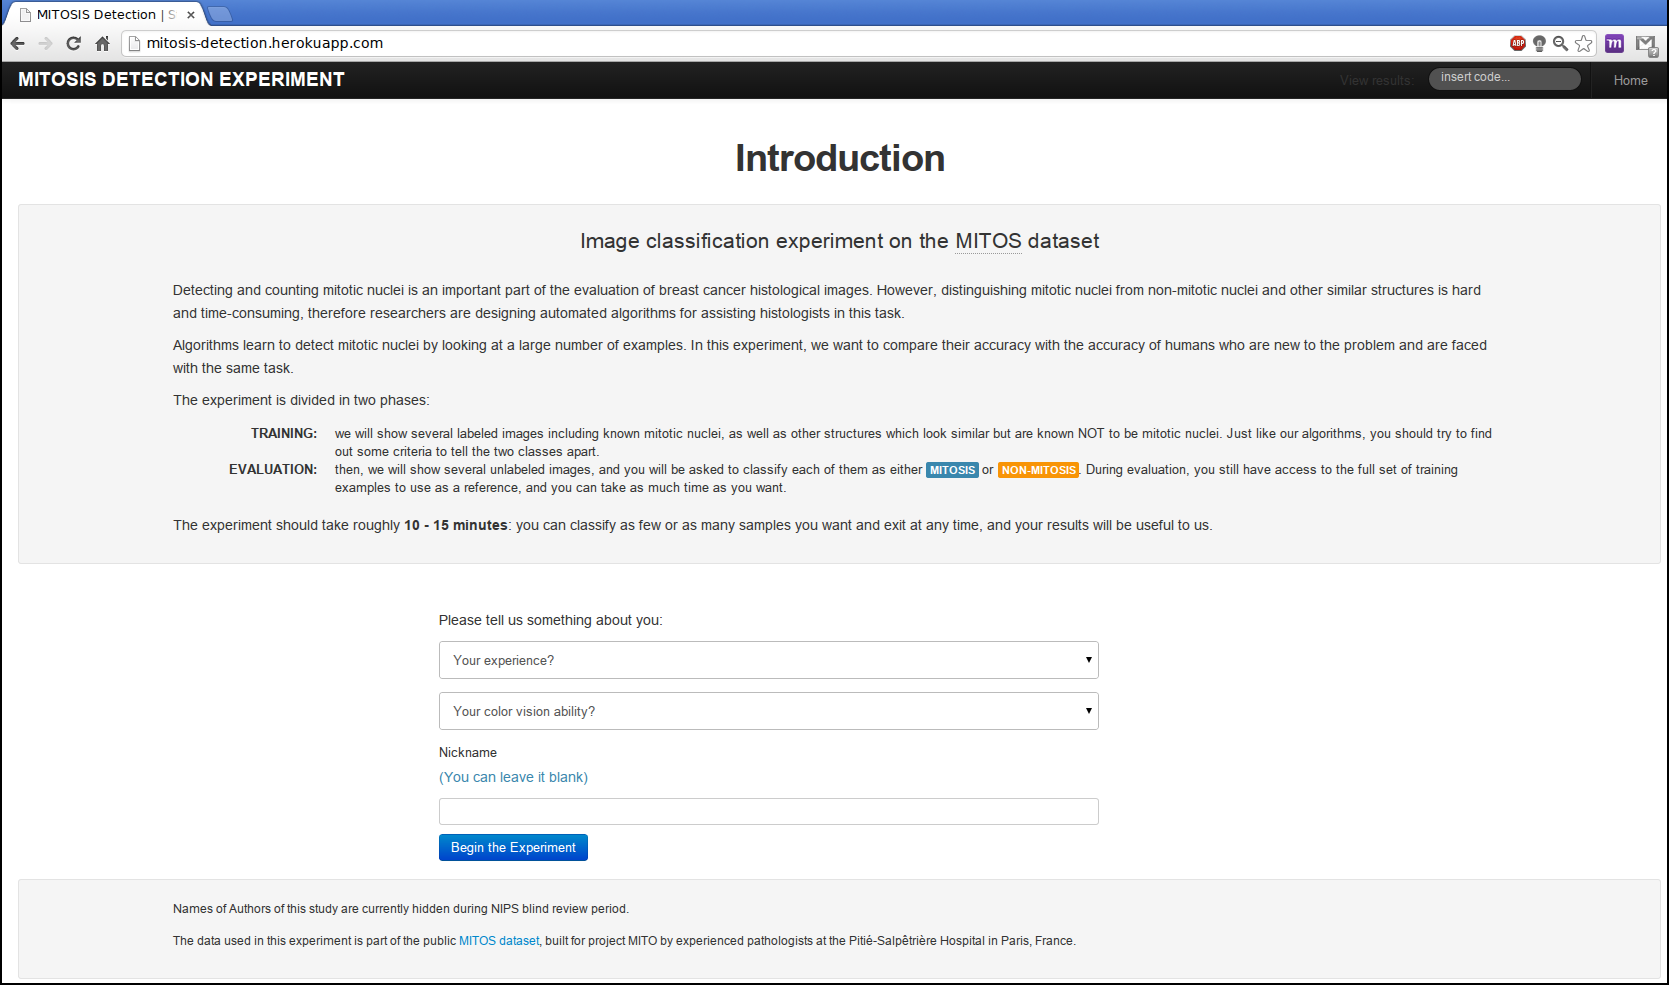
\includegraphics[width=0.98\textwidth]{./images/cr_MD_intro_mod.png}
    };
    \begin{scope}[x={(image.south east)},y={(image.north west)}]
      \coordinate (a) at (0,0);
      \coordinate (b) at (4,0);
      \draw[red, thick, decorate, decoration={brace, amplitude=8pt}] (0.25,0.12) -- (0.25,0.38)
	      node [midway,xshift=-20pt] {\small form};
    \end{scope}
\end{tikzpicture}
  \caption{Intro page}
  \label{ch5:fig1_intro}
\end{figure}  



\vspace{0.5cm}



\subsection{Training}

Once the user decides to participate, a new \textit{detection} entity is created and linked to a unique alphanumeric string that can be used to retrieve the summary of the performance.
The first step of the classification process is the \textit{training} phase, during which the subject is shown 216 labeled \textbf{C1} samples, 216 labeled \textbf{C0} samples, and
instructed to study them and devise some differentiating criteria (see Figure \ref{ch5:fig2_train}). The dataset is composed of the same images as the one used for automatic classification (see Section \ref{ch4:ds}).

\begin{figure}[!hbt]
  \centering
\begin{tikzpicture}
    \node[anchor=south west,inner sep=0] (image) at (0,0) {
      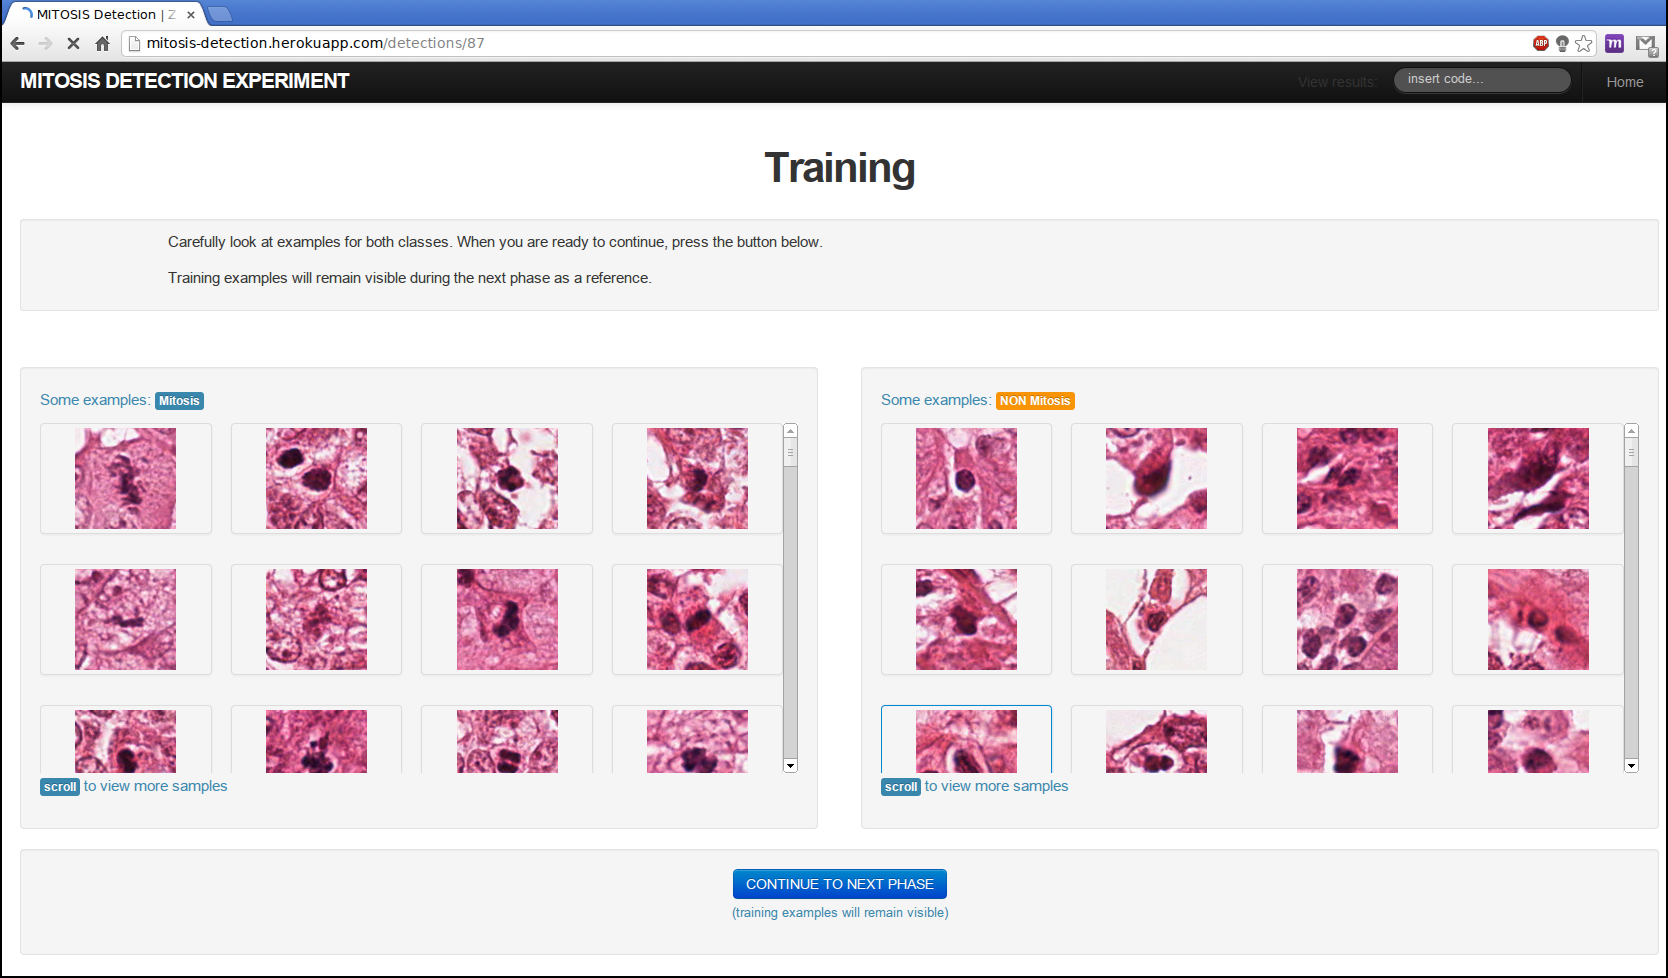
\includegraphics[width=0.87\textwidth]{./images/cr_MD_train_mod.png}
    };
    \begin{scope}[x={(image.south east)},y={(image.north west)}]
      \coordinate (a) at (0.0,0.15);
      \coordinate (b) at (0.0,0.63);
      \coordinate (c) at (1.0,0.15);
      \coordinate (d) at (1.0,0.63);
      
      \draw[red, thick, decorate, decoration={brace, amplitude=8pt}] (a) -- (b)
	      node [midway,xshift=-14pt] {\tiny C1};
      \draw[red, thick, decorate, decoration={brace, amplitude=8pt,mirror}] (c) -- (d)
	      node [midway,xshift=14pt] {\tiny C0};
    \end{scope}
\end{tikzpicture}
  \caption{Training page}
  \label{ch5:fig2_train}
\end{figure}  


\vspace{0.5cm}

\subsection{Evaluation}

During evaluation, the subject is presented with one evaluation sample at a time (randomly chosen among unseen ones), and asked to provide a classification as one of:
\begin{itemize}
 \item \textit{definitely mitosis}: $p(C1)=1.0$,
 \item \textit{probably mitosis}: $p(C1)=0.75$,
 \item \textit{probably non-mitosis}: $p(C1)=0.25$,
 \item \textit{definitely non-mitosis}: $p(C1)=0.0$,
\end{itemize}

During the evaluation phase, the whole training set remains visible for reference (see Figure \ref{ch5:fig3_eval}). The number of classification options has been chosen so that the user is led to make
a commitment over the type of current image: towards \textbf{C0} or towards \textbf{C1}.

\begin{figure}[!hbt]
  \centering
\begin{tikzpicture}
    \node[anchor=south west,inner sep=0] (image) at (0,0) {
      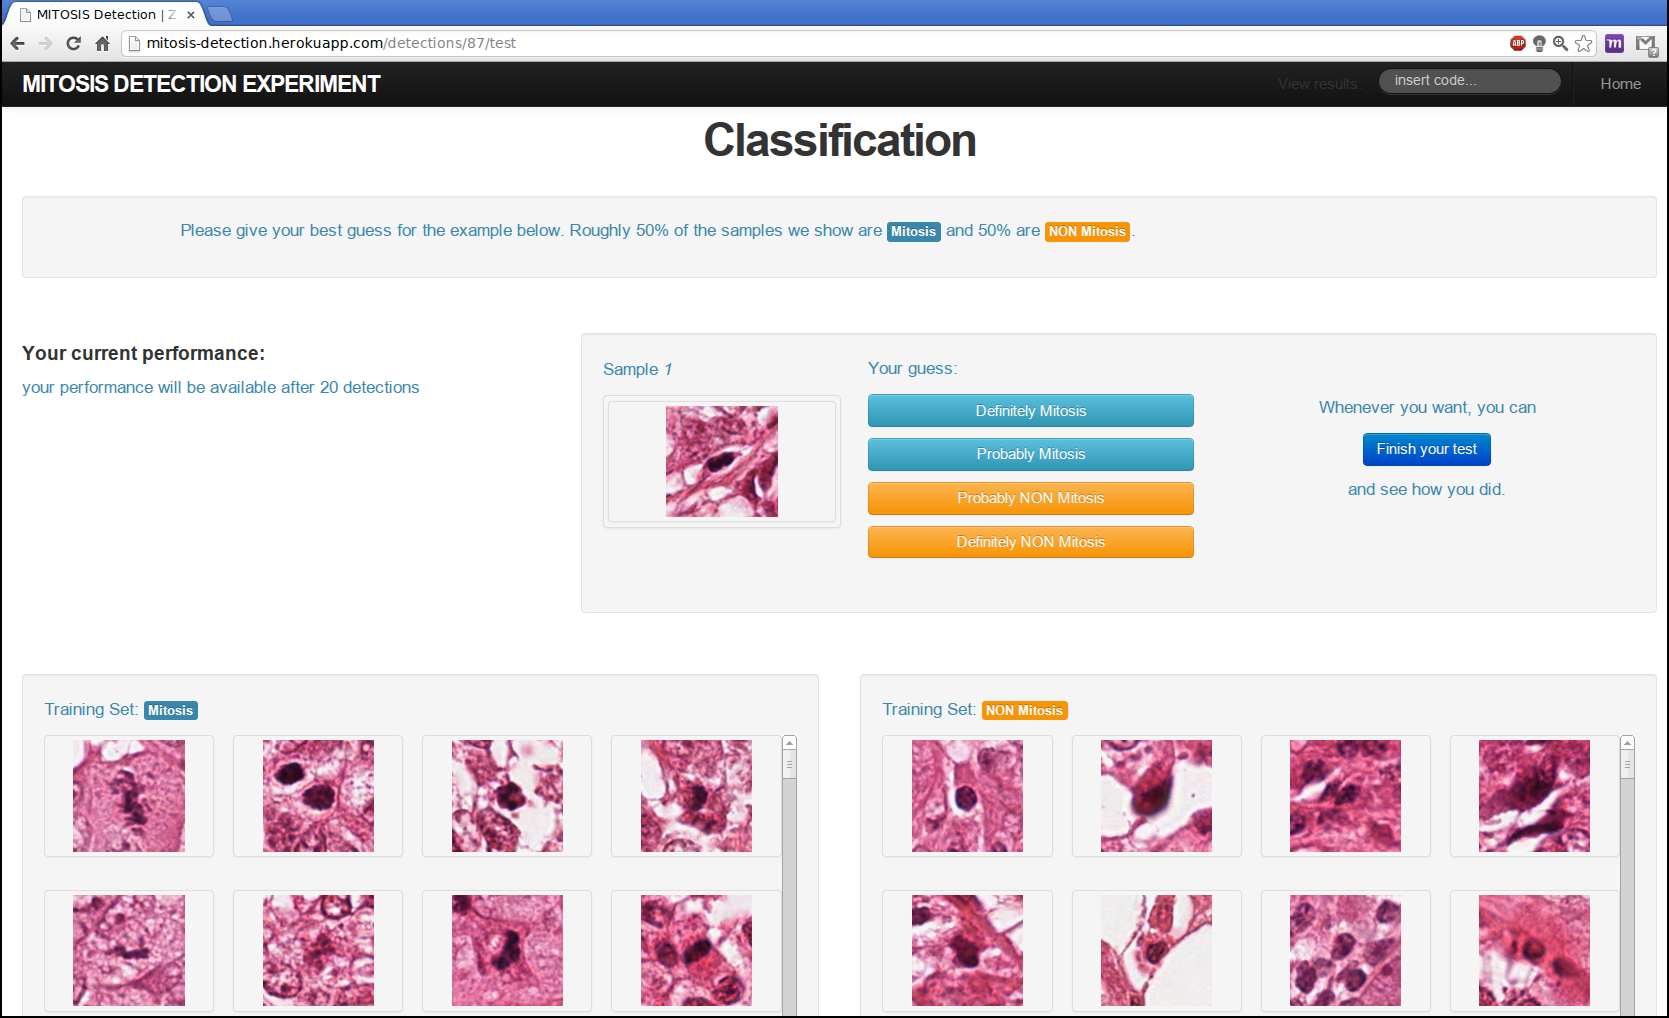
\includegraphics[width=0.88\textwidth]{./images/cr_MD_eval0_mod.png}
    };
    \begin{scope}[x={(image.south east)},y={(image.north west)}]
      \coordinate (a) at (0.02,0.0);
      \coordinate (b) at (0.02,0.34);
      \coordinate (c) at (0.99,0.0);
      \coordinate (d) at (0.99,0.34);
      \coordinate (e) at (0.345,0.4);
      \coordinate (f) at (0.345,0.67);
      \coordinate (g) at (0.92,0.4);
      \coordinate (h) at (0.92,0.67);      
      
      
      \draw[red, thick, decorate, decoration={brace, amplitude=8pt}] (a) -- (b)
	      node [midway,xshift=-14pt] {\tiny C1};
      \draw[red, thick, decorate, decoration={brace, amplitude=8pt,mirror}] (c) -- (d)
	      node [midway,xshift=14pt] {\tiny C0};
      \draw[red, thick, decorate, decoration={brace, amplitude=6pt}] (e) -- (f)
	      node [midway,xshift=-18pt,yshift=0.0] {\tiny \textbf{\textit{sample}}};
      \draw[red, thick, decorate, decoration={brace, amplitude=6pt,mirror}] (g) -- (h)
	      node [midway,xshift=16.5pt,yshift=-0.05] {\tiny \textbf{\textit{class}}};    \end{scope}
\end{tikzpicture}
  \caption{Evaluation page}
  \label{ch5:fig3_eval}
\end{figure}  

A number of design decisions are taken in order to balance the trade-off between test fairness and subject engagement. Most importantly, the user is given
immediate feedback as to whether the last decision was correct or wrong (see Figure \ref{ch5:fig4_fb}): on one hand, this encourages continuous learning while the evaluation is taken and
makes users much more willing to improve and fine-tune their strategies; on the other hand, subjects can count on a growing training set, which gives them an
unfair advantage over algorithms.

\begin{figure}[!hbt]
  \centering
    \subfigure[positive Feedback]{
	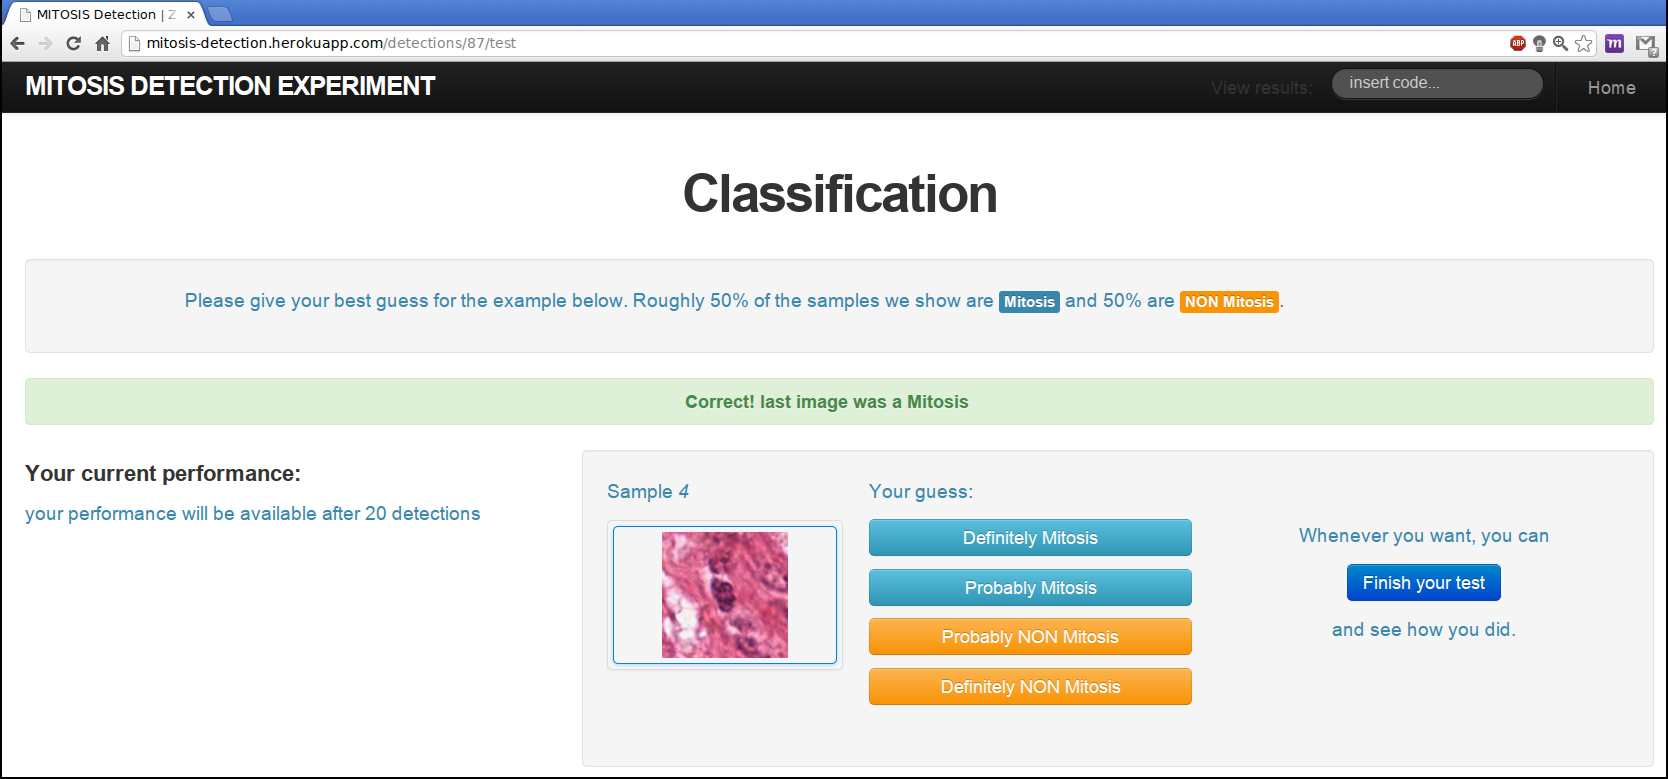
\includegraphics[width=0.87\textwidth]{./images/cr_MD_eval_OK_mod.png}
	\label{ch5:fig4:a}
    }\\
    %\hspace{1mm}
    \subfigure[negative Feedback]{
      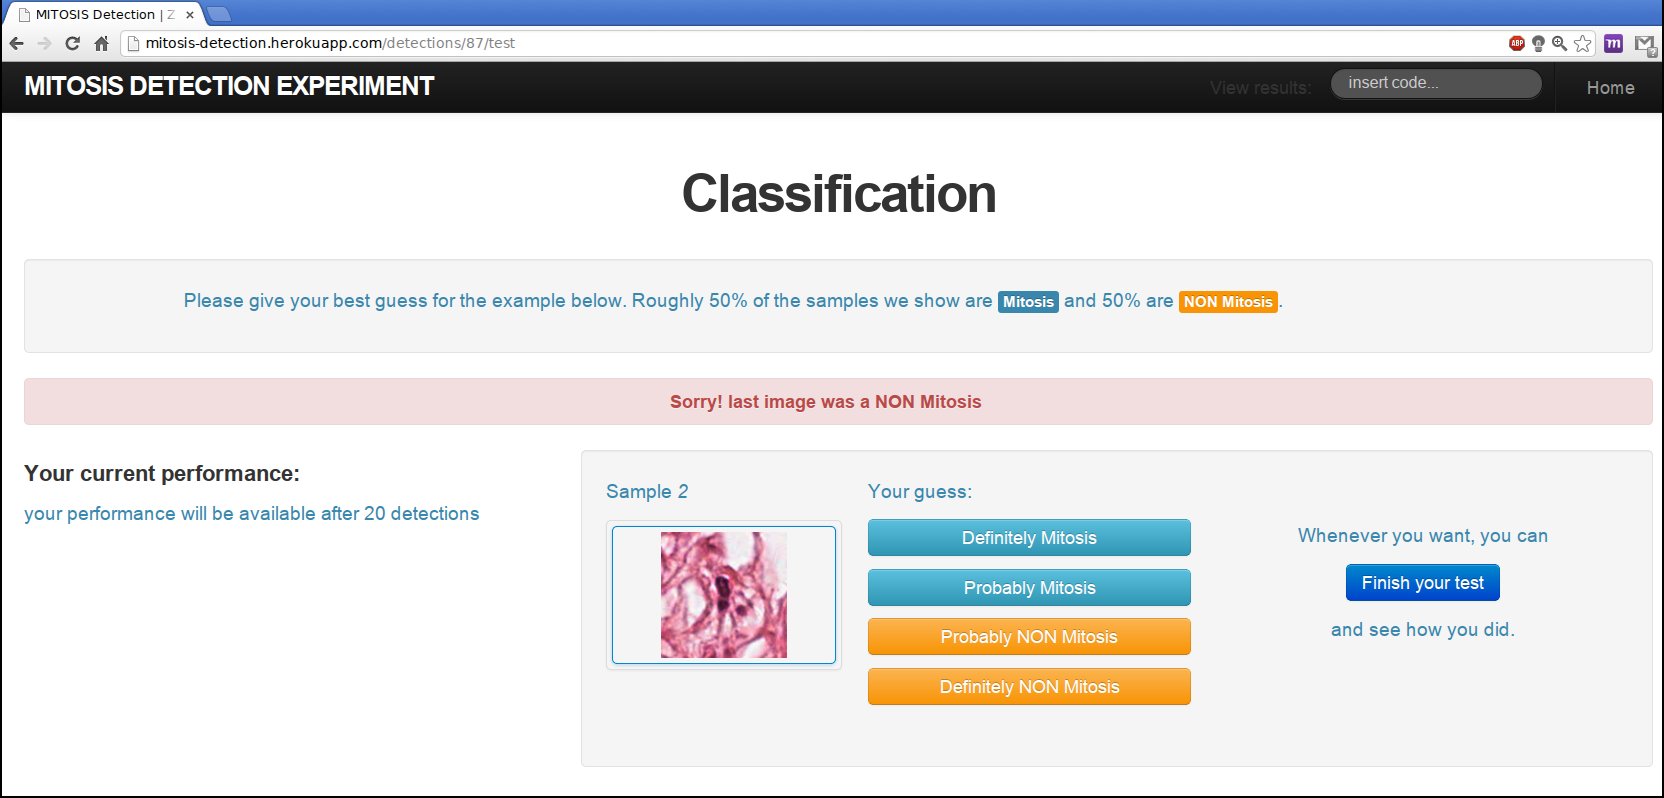
\includegraphics[width=0.87\textwidth]{./images/cr_MD_eval_KO_mod.png}
      \label{ch5:fig4:b}
    }
    \caption{Examples of classification feedback}
    \label{ch5:fig4_fb}
\end{figure}


In addition, subjects are allowed to finish the test at any time, the ones who reach a minimum of 20 classifications are shown their
current average accuracy, as illustrated in Figure \ref{ch5:fig5_perf}.

\begin{figure}[!hbt]
  \centering
\begin{tikzpicture}
    \node[anchor=south west,inner sep=0] (image) at (0,0) {
      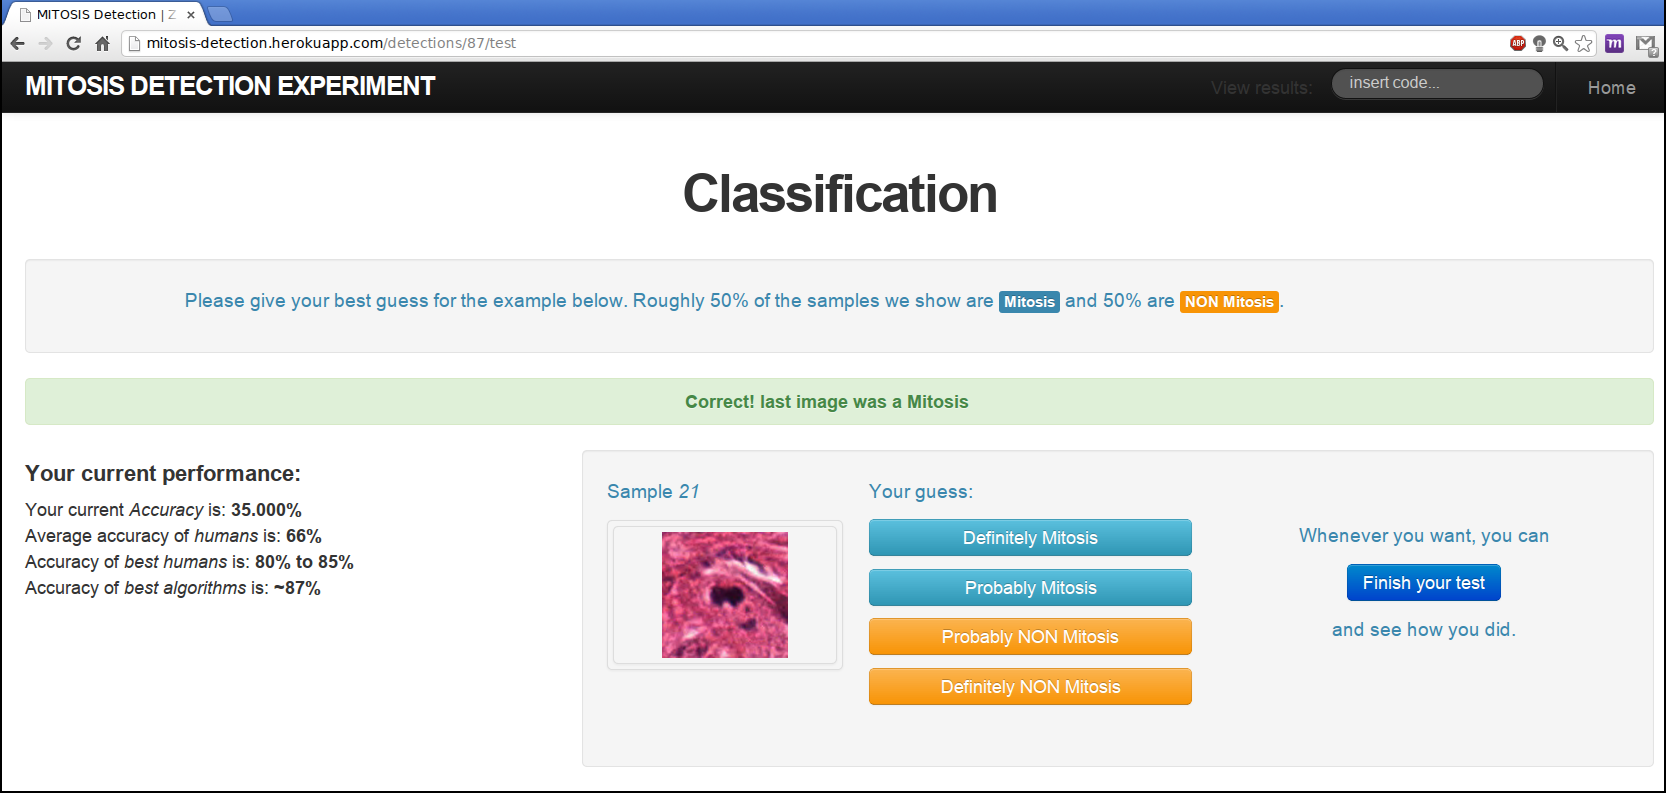
\includegraphics[width=0.87\textwidth]{./images/cr_MD_eval_act_perf_mod.png}
    };
    \begin{scope}[x={(image.south east)},y={(image.north west)}]
      \coordinate (a) at (0.0,0.2);
      \coordinate (b) at (0.23,0.46);
      
      \draw[red,ultra thick,rounded corners] (a) rectangle (b);
    \end{scope}
\end{tikzpicture}
  \caption{Current performance}
  \label{ch5:fig5_perf}
\end{figure}  

\vspace{0.5cm}


\subsection{Comments}

After concluding the classifications, the subject can write his opinions about the classification criteria that he devised during the process (see Figure \ref{ch5:fig6_comm}).

% \begin{figure}[!hbt]
%   \centering
%     \begin{tikzpicture}
%       \node[anchor=south west,inner sep=0] (image) at (0,0) {
% 	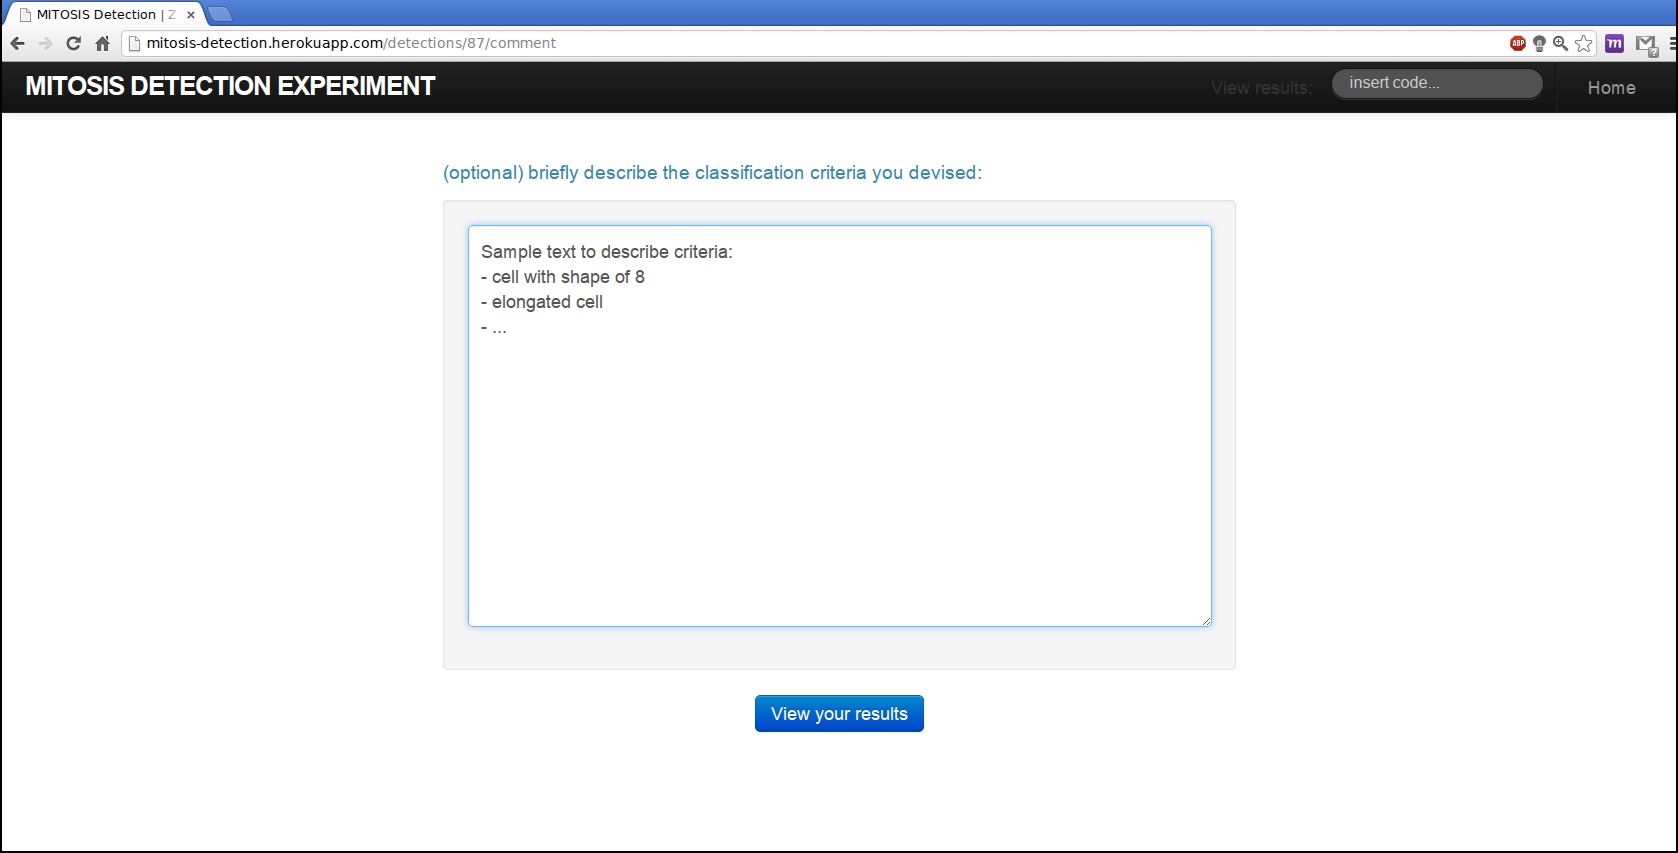
\includegraphics[width=0.92\textwidth]{./images/cr_MD_comments_mod.png}
%     };
%     \begin{scope}[x={(image.south east)},y={(image.north west)}]
%       \coordinate (a) at (0.0,0.0);
%       \coordinate (b) at (1.0,1.0);
%       
%       \draw[black,thin] (a) rectangle (b);
%     \end{scope}
% \end{tikzpicture}
%   \caption{Comment page}
%   \label{ch5:fig6_comm}
% \end{figure}  

\begin{figure}[!hbt]
  \centering
	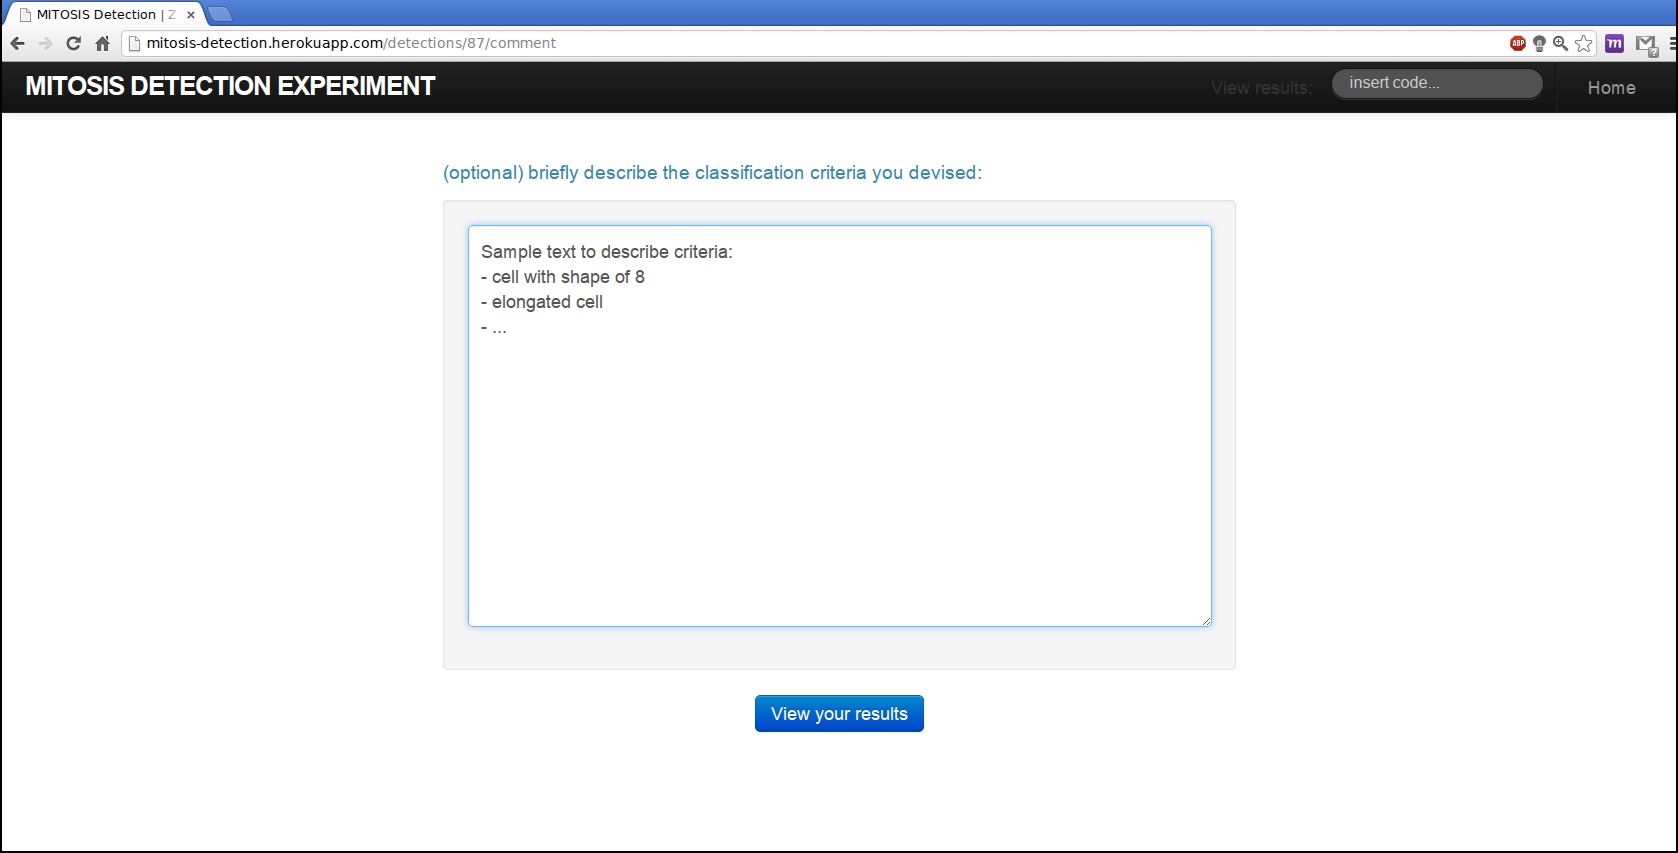
\includegraphics[width=0.92\textwidth]{./images/cr_MD_comments_mod.png}
  \caption{Comment page}
  \label{ch5:fig6_comm}
\end{figure}  


\vspace{0.5cm}

\subsection{Performances}

Finally, the user can review his overall performance, viewing his \textit{confusion matrix}, his \textit{accuracy}, \textit{sensitivity} and \textit{specificity} (as described in Section \ref{ch3:perf}).
The results page is shown in Figure \ref{ch5:fig7_res}.

% \begin{figure}[!hbt]
%   \centering
%     \begin{tikzpicture}
%       \node[anchor=south west,inner sep=0] (image) at (0,0) {
% 	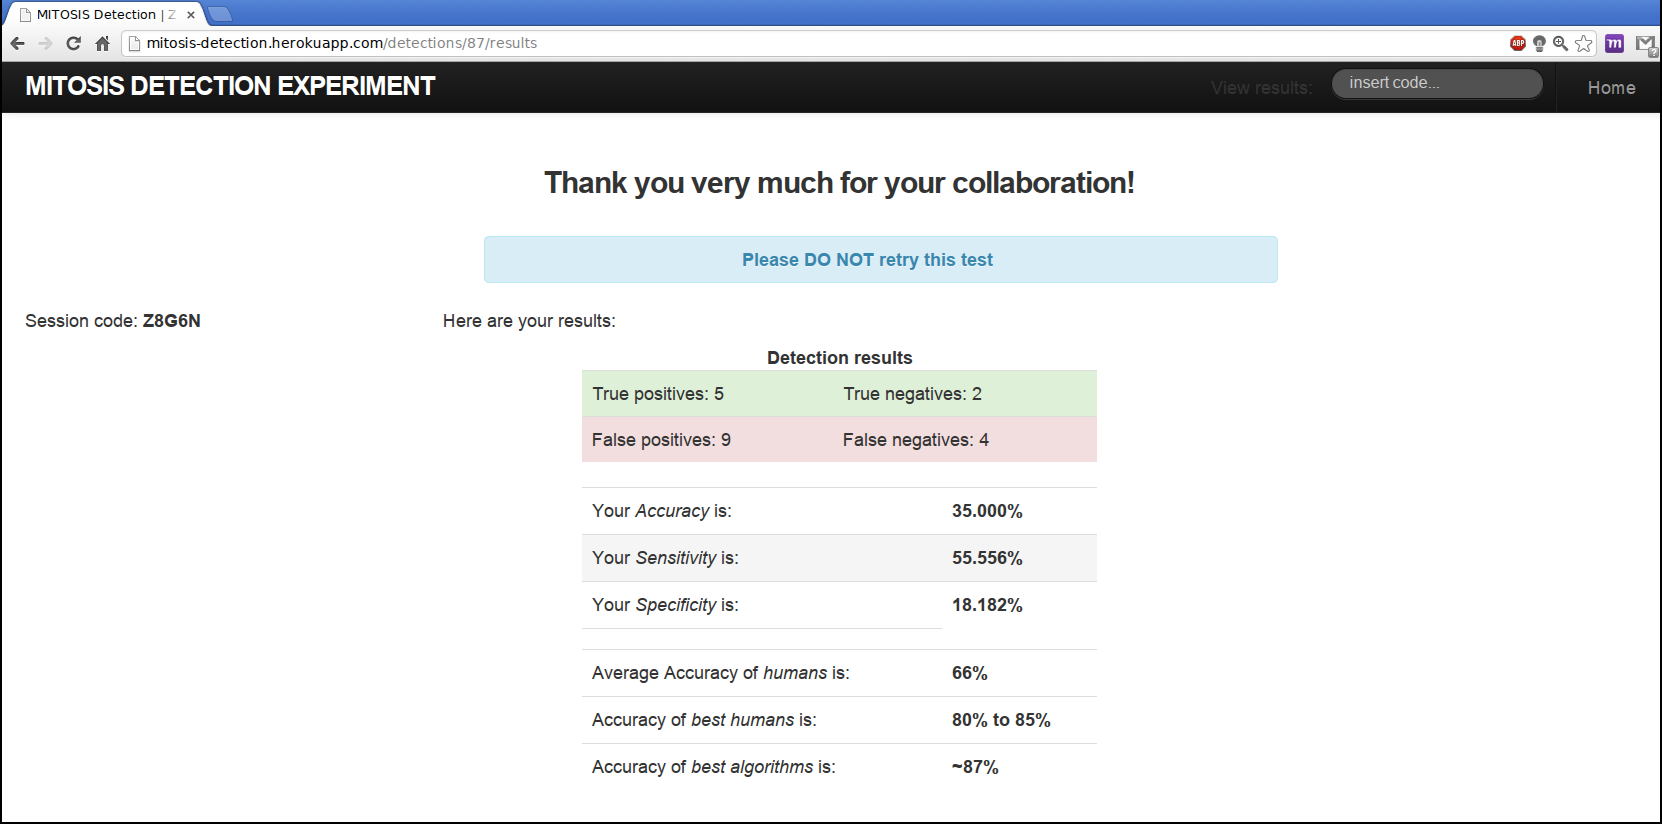
\includegraphics[width=0.92\textwidth]{./images/cr_MD_user_res_mod.png}
%     };
%     \begin{scope}[x={(image.south east)},y={(image.north west)}]
%       \coordinate (a) at (0.0,0.0);
%       \coordinate (b) at (1.0,1.0);
%       
%       \draw[black,thin] (a) rectangle (b);
%     \end{scope}
% \end{tikzpicture}
%   \caption{user results page}
%   \label{ch5:fig7_res}
% \end{figure}  

\begin{figure}[!hbt]
  \centering
	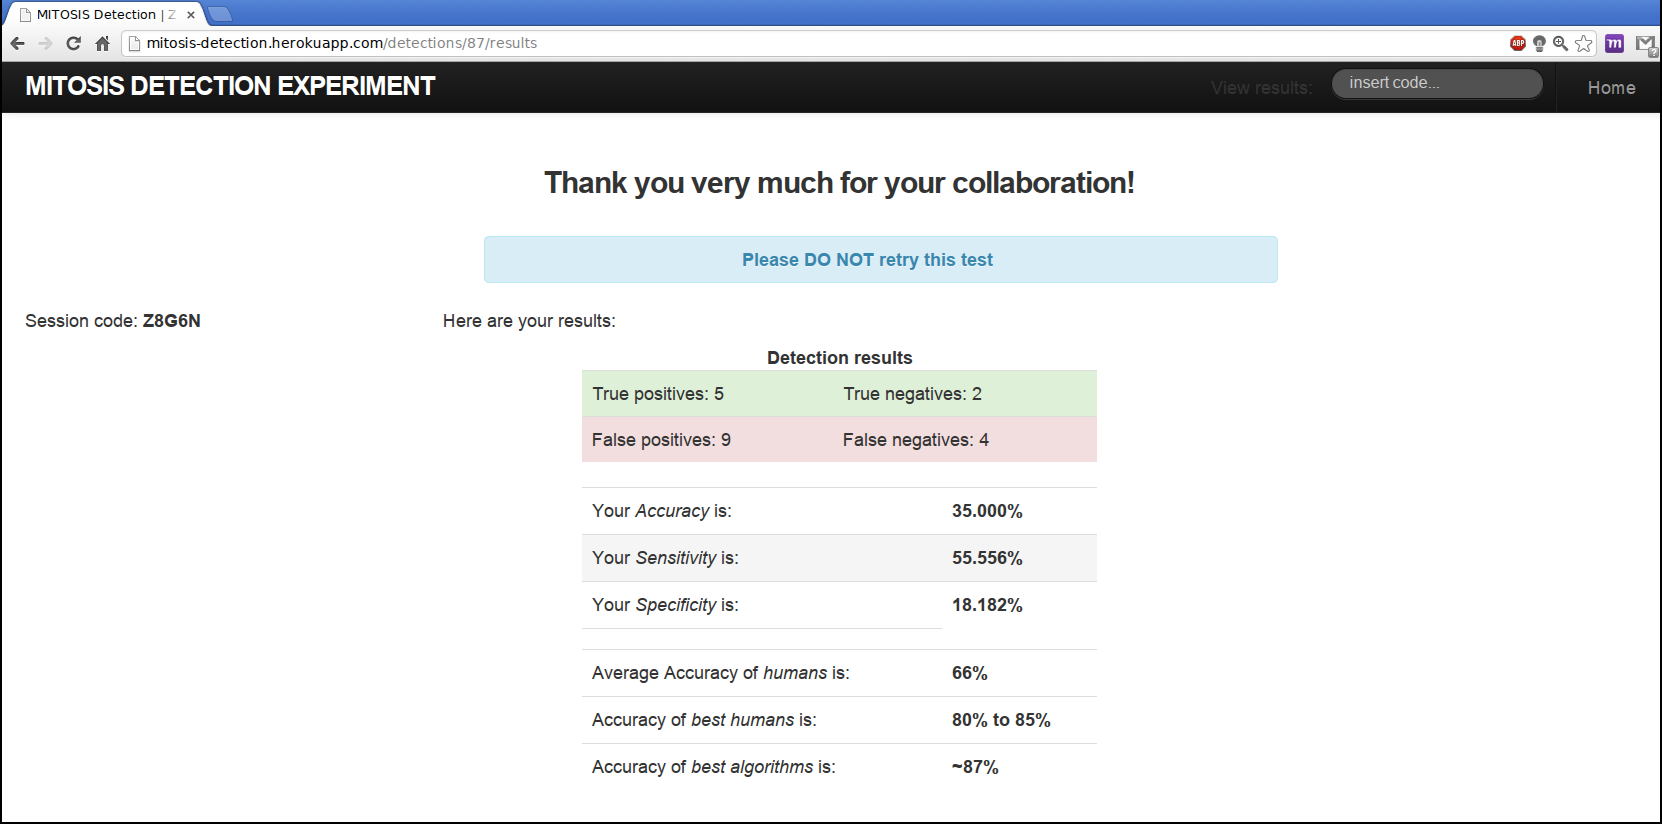
\includegraphics[width=0.92\textwidth]{./images/cr_MD_user_res_mod.png}
  \caption{user results page}
  \label{ch5:fig7_res}
\end{figure}  

\vspace{0.5cm}


\section{Data collection}

In a not directly reachable web-page, it is possible to view and download all the data collected by the site. A table, shown in Figure \ref{ch5:fig8_data},
reports the main information of all the concluded classifications.\\
It is possible to download (see Figure \ref{ch5:fig9_dl}) two \texttt{.csv} files. One (\texttt{images.csv}) summarizes the dataset, for each image patch it gives:
\begin{itemize}
 \item \textit{id}: a unique number identifying each image,
 \item \textit{image}: the name of the image from which the patch has been taken,
 \item \textit{coordinates}: the $(x,y)$ coordinates of the center in the image,
 \item \textit{type}: if the image is \textbf{C1} or \textbf{C0}.
\end{itemize}

\noindent The other file (\texttt{users.csv}) summarizes the classifications. Each detection starts with a line beginning with the keyword \texttt{USER}.
The first line of a detection reports the information concerning user and detection:

\begin{itemize}
 \item nickname, user type and color ability of the user,
 \item timestamp of the detection,
 \item number of detections: \Glspl{TP}, \Glspl{TN}, \Glspl{FP}, \Glspl{FN},
 \item \textit{ID} of the detection.
\end{itemize}

\noindent The line concerning the classified images reports:

\begin{itemize}
 \item \textit{id}: the unique number identifying the patch,
 \item \textit{image}: the name of the image from which the patch has been taken,
 \item \textit{coordinates}: the $(x,y)$ coordinates of the center in the image,
 \item \textit{type}: if the image is \textbf{C1} or \textbf{C0}.
 \item \textit{classification}: how the user classified the image: $\{0.0, 0.25, 0.75, 1.0\}$,
 \item \textit{time}: how many seconds took the user to decide.
\end{itemize}

\noindent Finally it is possible to view all the comments left by the users (see Figure \ref{ch5:fig10_comm}).


\begin{figure}[!hbt]
  \centering
	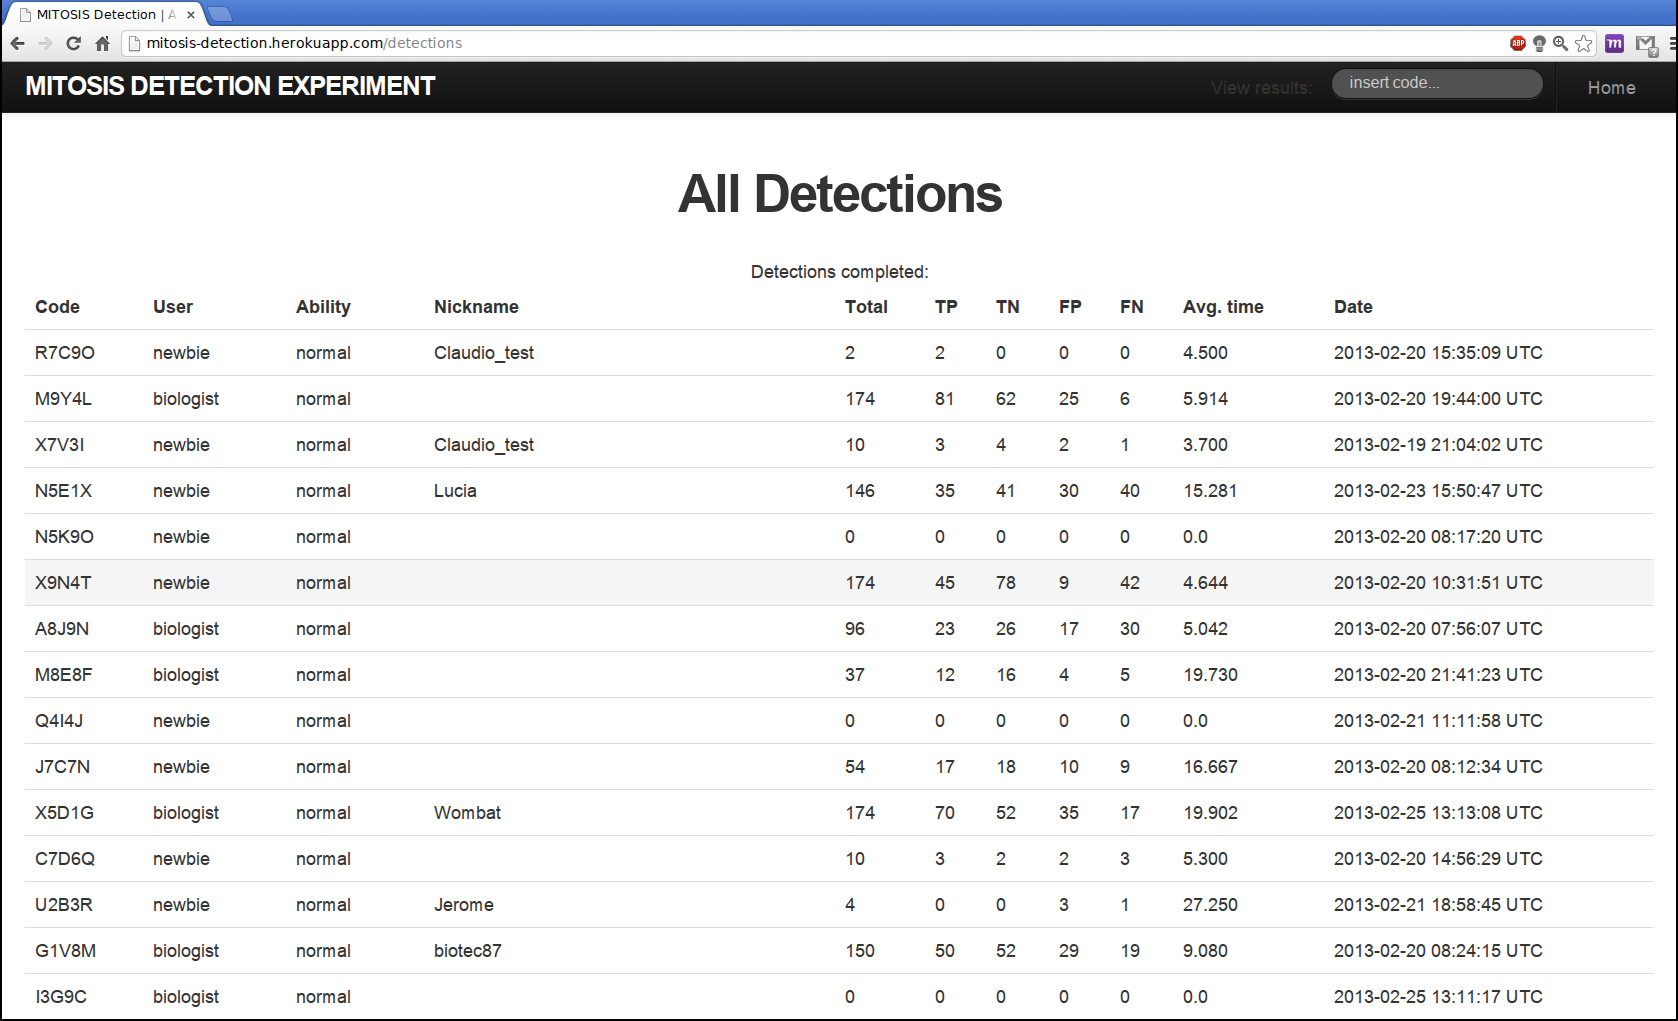
\includegraphics[width=0.92\textwidth]{./images/cr_MD_data_all_mod.png}
  \caption{Overall results page}
  \label{ch5:fig8_data}
\end{figure}

\begin{figure}[!hbt]
  \centering
	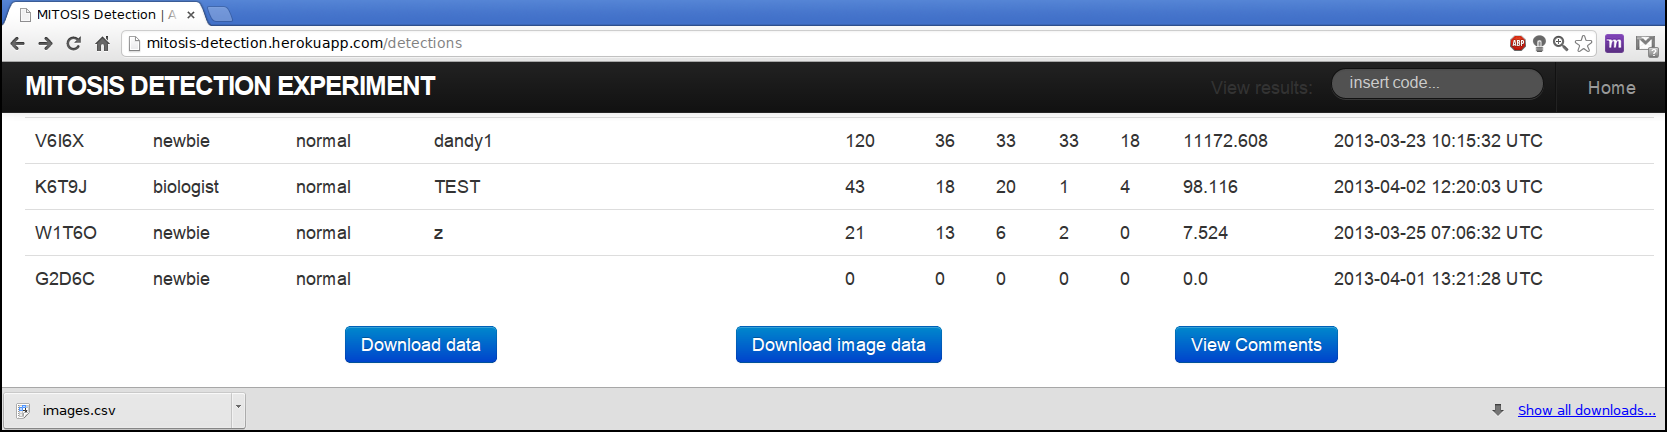
\includegraphics[width=0.92\textwidth]{./images/cr_MD_data_dl_mod.png}
  \caption{Download buttons}
  \label{ch5:fig9_dl}
\end{figure}

\begin{figure}[!hbt]
  \centering
	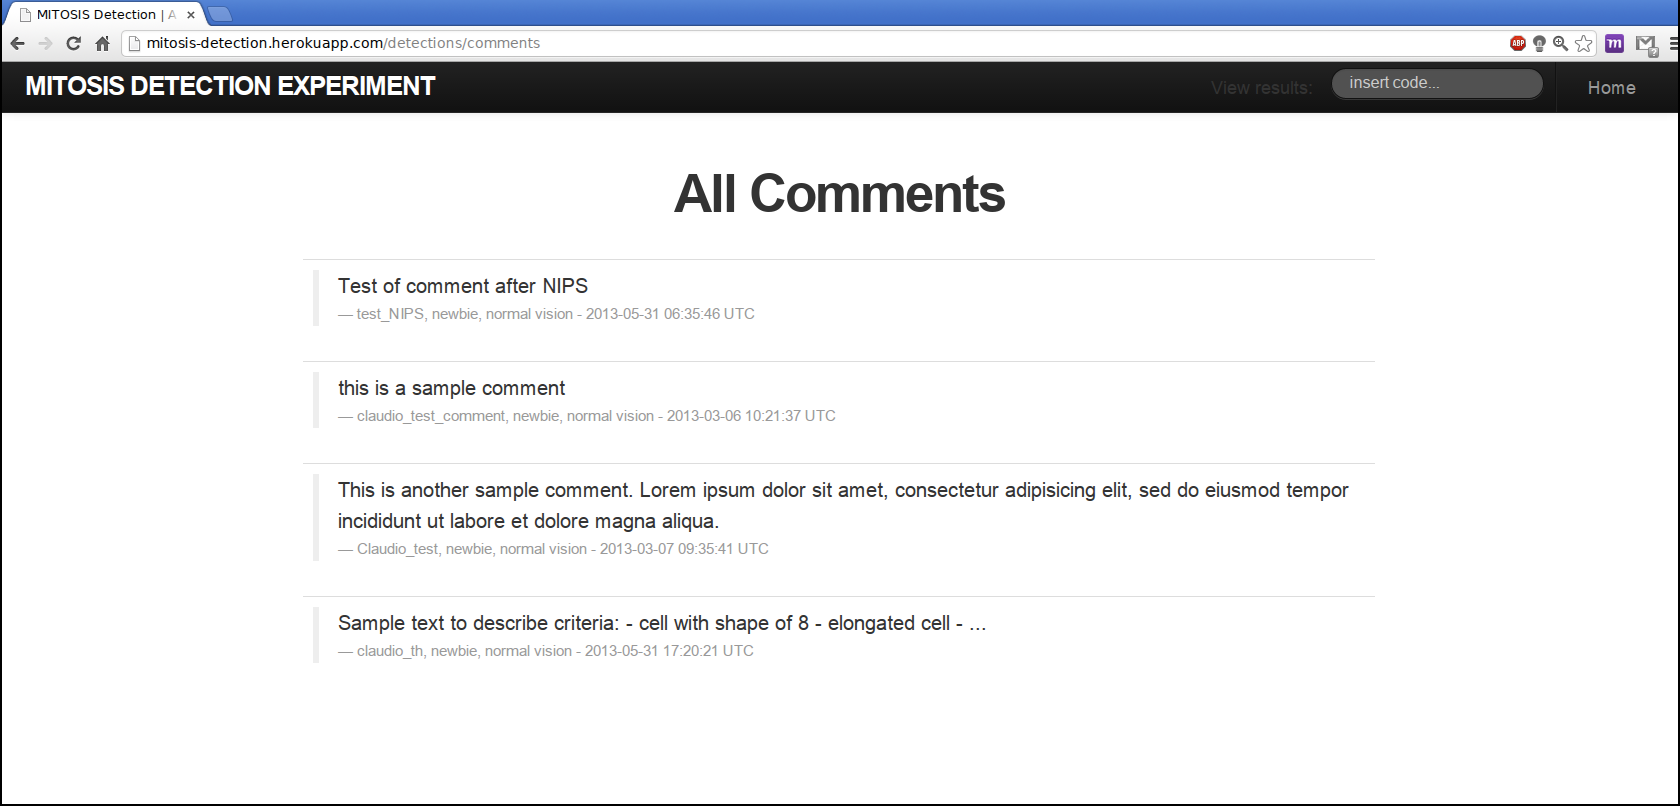
\includegraphics[width=0.92\textwidth]{./images/cr_MD_data_comments_mod.png}
  \caption{User comments}
  \label{ch5:fig10_comm}
\end{figure}

% 
% \begin{figure}[!hbt]
%   \centering
%     \begin{tikzpicture}
%       \node[anchor=south west,inner sep=0] (image) at (0,0) {
% 	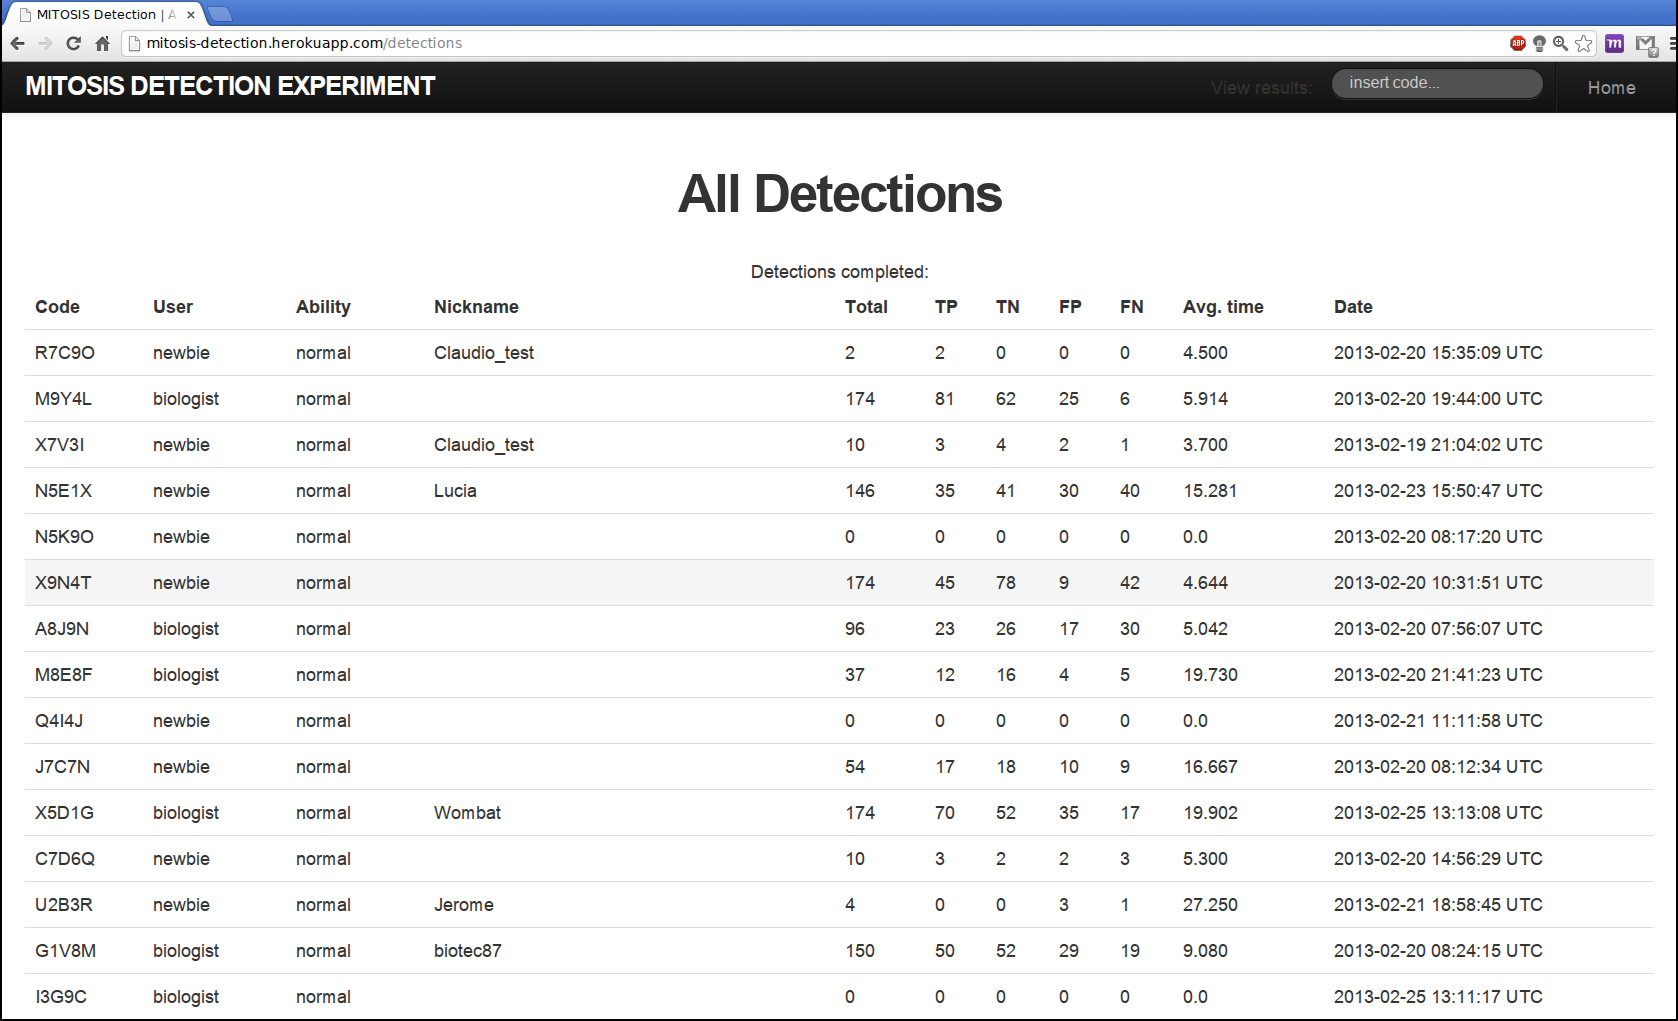
\includegraphics[width=0.92\textwidth]{./images/cr_MD_data_all_mod.png}
%     };
%     \begin{scope}[x={(image.south east)},y={(image.north west)}]
%       \coordinate (a) at (0.0,0.0);
%       \coordinate (b) at (1.0,1.0);
%       
%       \draw[black,thin] (a) rectangle (b);
%     \end{scope}
% \end{tikzpicture}
%   \caption{Overall results page}
%   \label{ch5:fig8_data}
% \end{figure}
% 
% \begin{figure}[!hbt]
%   \centering
%     \begin{tikzpicture}
%       \node[anchor=south west,inner sep=0] (image) at (0,0) {
% 	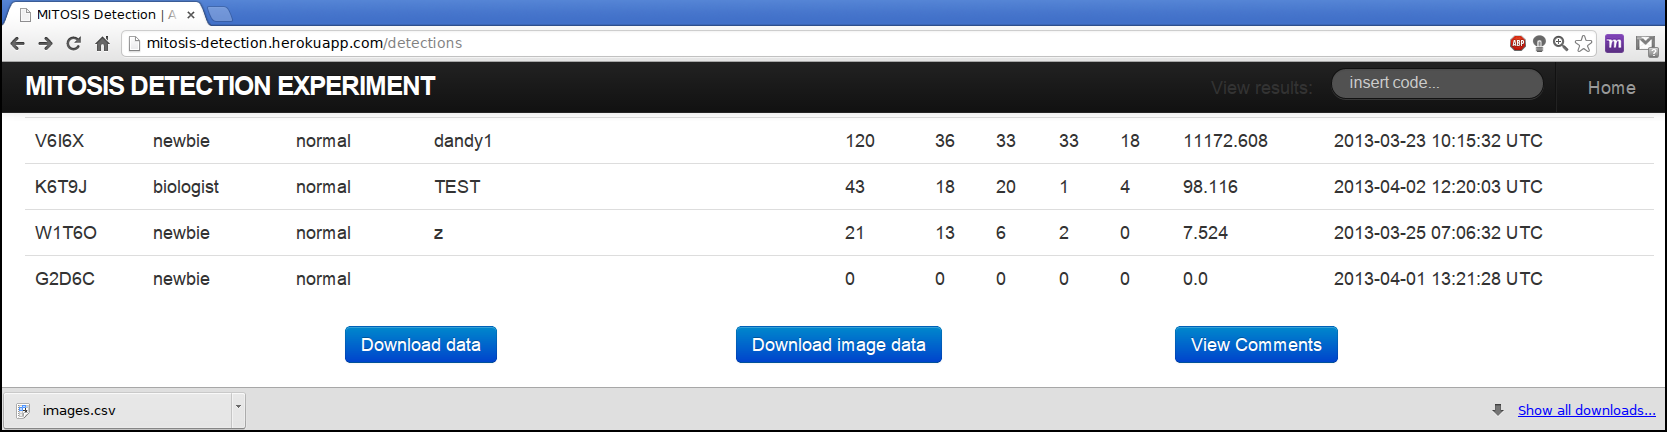
\includegraphics[width=0.92\textwidth]{./images/cr_MD_data_dl_mod.png}
%     };
%     \begin{scope}[x={(image.south east)},y={(image.north west)}]
%       \coordinate (a) at (0.0,0.0);
%       \coordinate (b) at (1.0,1.0);
%       
%       \draw[black,thin] (a) rectangle (b);
%     \end{scope}
% \end{tikzpicture}
%   \caption{Download buttons}
%   \label{ch5:fig9_dl}
% \end{figure}
% 
% \begin{figure}[!hbt]
%   \centering
%     \begin{tikzpicture}
%       \node[anchor=south west,inner sep=0] (image) at (0,0) {
% 	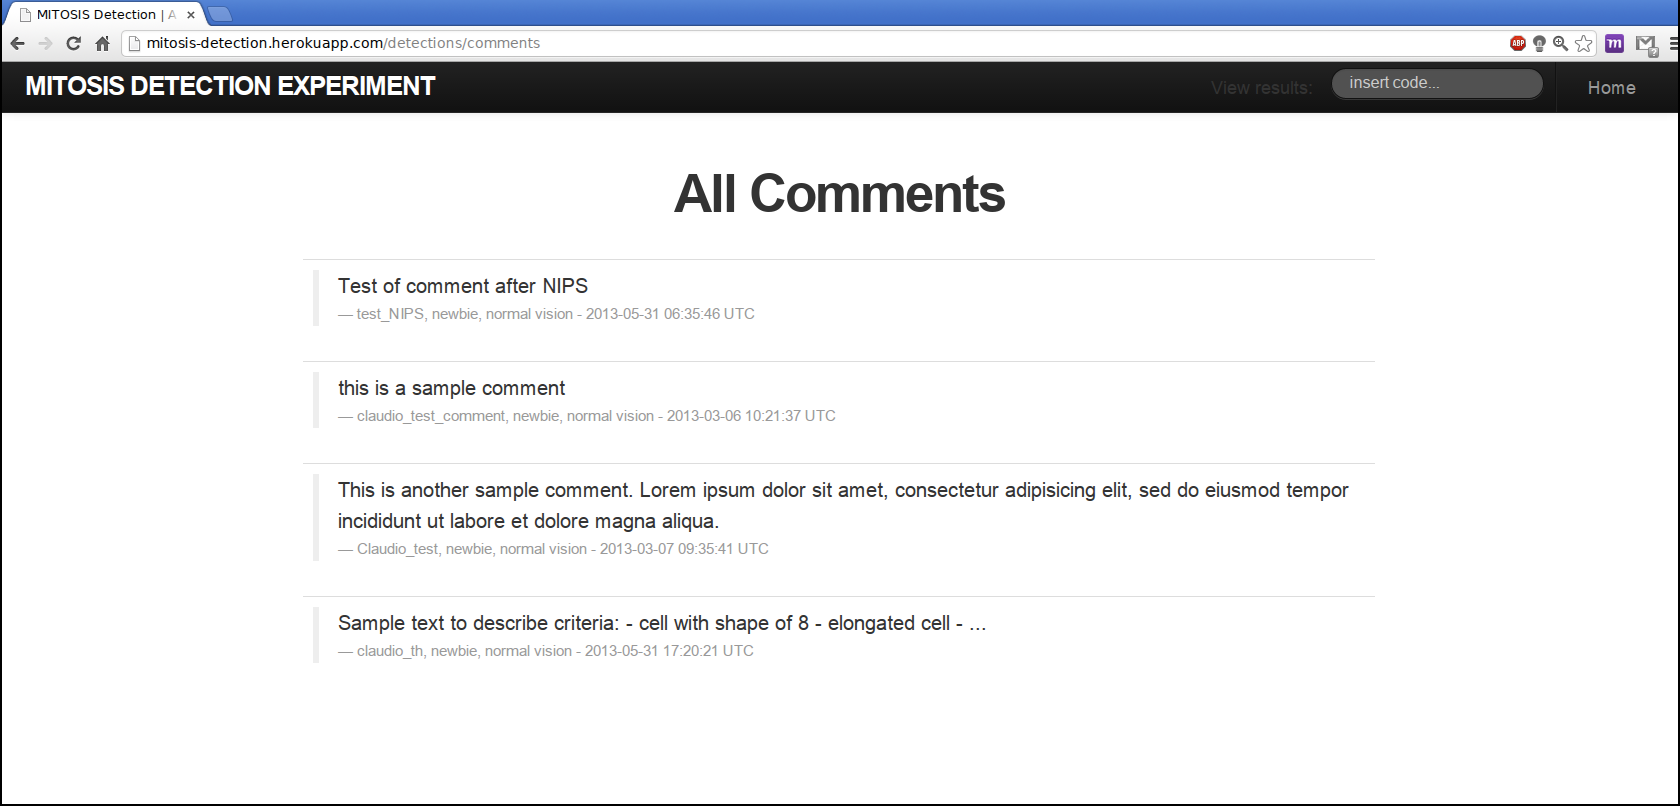
\includegraphics[width=0.92\textwidth]{./images/cr_MD_data_comments_mod.png}
%     };
%     \begin{scope}[x={(image.south east)},y={(image.north west)}]
%       \coordinate (a) at (0.0,0.0);
%       \coordinate (b) at (1.0,1.0);
%       
%       \draw[black,thin] (a) rectangle (b);
%     \end{scope}
% \end{tikzpicture}
%   \caption{User comments}
%   \label{ch5:fig10_comm}
% \end{figure}

\vspace{0.5cm}

\section{Source Code}
The entire project source code is maintained at the following repository:\\
\url{https://github.com/Ccaccia73/tydes}.